Durch die intensive Interaktion der Bereiche Entwicklung und Betrieb müssen unterschiedliche organisatorische und kulturelle Veränderungen durchgeführt werden, damit die DevOps-Kultur etabliert werden kann. 

In diesem Abschnitt wird zunächst auf die wesentlichen Bestandteile und die Ziele der Kultur eingegangen, damit die Zusammenarbeit zwischen den beiden Bereichen gelingt.

In diesem Rahmen baut DevOps auf den Hauptprinzipien, als das Model der \textit{'The Three Ways'} auf, die von dem Autor und Erfinder des DevOps-Ansatzes Gene Kim \cite{kim_devops-handbuch_2017} definiert wurden. 
\dwi{ist das glasklar belegbar, das dieser Kim der urheber/namensgeber ist das ist eine starke aussage, die ich
ansonsten weiter oben im kontext 'devops geht zurück auf Gene Kim und XYZ'}

Dieses Model der drei Wege bilden die zugrunde liegenden Prinzipien von DevOps ab, indem das Verhalten und die Muster von DevOps näher beschrieben werden. \cite[S. 9 - 44]{kim_devops-handbuch_2017}, \cite{kim_three_2012}  

Zunächst bildet der erste Weg die Grundlage für DevOps ab und betont die Leistung des gesamten Systems, im Gegensatz zur Leistung eines einzelnen Teams, Silos oder Abteilungen. 

Der Fokus liegt hierbei auf einem schnellen Arbeitsfluss des gesamten Systems, der durch die IT ermöglicht wird. 

In diesem Sinne müssen sich Opimierungen auf das gesamte System auswirken und sich nicht auf einen bestimmten Bestandteil beziehen. 

Das Ergebnis einer lokalen Veränderung zeigt meist keine Wirkung und würde im schlechteren Fall eine Verschlimmerung der Gesamtsituation herbeiführen. \cite[S. 252]{tiemeyer_handbuch_2021} 

Zudem sollte eine Veränderung, die ausschließlich stromab eine Verbesserung innerhalb des Wertestroms zeigt und stromab stark erschwert, kann nicht förderlich für das gesamte System sein. \cite[S. 252]{tiemeyer_handbuch_2021}
\dwi{und stromab stark erschwert ?}

Den Anfang stellt der Kunde dar, über die Entwicklung bis hin zu den Operations.

Dabei wird das Produkt, basierend auf den identifizierten Anforderungen des Kundenanforderungen, von der Entwicklung erstellt und in den Betrieb übergeben, wo das Ergebnis dem Kunden ausgeliefert wird.\cite[S. 12]{halstenberg_devops_2020} 

Der erste Schritt greift zudem den Grundgedanken des Lean-Ansatzes auf, indem ein Fehler nicht an nachfolgede Arbeitseinheiten weitergegeben werden darf um damit einen verbesserter Arbeitsfluss aufrecht gehalten werden kann. \cite[S. 252]{tiemeyer_handbuch_2021}  

Daher sind alle Arbeiten während dieses Schrittes sichtbar und in kleinen Aufgaben aufgeteilt, die in bestimmten Intervallen ausgeführt werden. 

Zu den Zielen des Ersten Weges gehört, dass bekannte Fehler an nachfolgende Arbeitsplätze nicht weitergegeben werden, dass eine lokale Optimierung niemals zu einer globalen Verschlechterung führt und dass versucht wird, ein tiefes Verständnis des gesamten Systems zu erlangen. \cite{kim_three_2012}  

\begin{figure}[h]
    \centering
    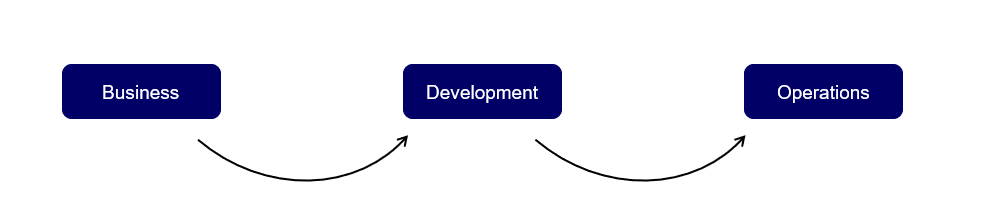
\includegraphics[scale=0.6]{Bilder/First Way.png}
    \caption{Der erste Weg: Systemdenken \cite{kim_three_2012}}
\end{figure}

Der zweite Weg beschreibt das Gestalten von effizienten Feedbackschleifen, um einerseits Fehler schnell und frühzeitig zu erkennen und zu beheben und andererseits den Prozess durchgängig im Auge zu behalten.

Der zweite Schritt stellt den eigentlichen zentralen Ansatzes von DevOps dar, wobei das Feedback von verschiedener Natur sein kann. \cite[S. 254]{tiemeyer_handbuch_2021} 

Dies sollte sowohl auf Seiten von einzelnen Teams untereinander als auch zwischen Entwicklung und Betrieb eingebettet werden. \cite[S. 94]{ravichandran_devops_2016}

Denn je schneller Probleme oder Auswirkungen kommuniziert werden, desto besser kann eine Vorgehensweise festgelegt werden. 

Damit soll verhindert werden, dass Fehler kein zweites Mal auftreten, sich kontinuierlich aufbauen können und sich möglicherweise auf neue Aufgaben auswirken. 

Durch die erleicherte Kommunikation zwischen den einzelnen Teamitgliedern als Basis von Feedbackschleifen, führt dies zu einer erhöhten Effizienz des gesamten Teams. 

Zudem können neue oder geänderte Kundenanforderungen mittels schneller Feedbackschleifen an die Entwicklung weitergegeben werden, um möglichst zeitnah die geeigneten Maßnahmen treffen zu können.
\dwi{woher kommen die kundenanforderungen? das kann ja fachlich neu oder erkenntnisse aus dem betrieb/nutzung der anwendung sein. letzteres ist ja hier gemeint, das sollte ggf klargestellt werden.}

Entscheidend ist, dass das Hinzufügen weiterer Kontrollschritte und schwerfällige Genehmigungsprozesse innerhalb großer Arbeitssyssteme die Wahrscheinlichkeit für zukünftige Fehler maßgeblich erhöht. \cite[S. 31]{kim_devops-handbuch_2017} 

Daher müssen DevOps-Teams die Freiheit haben, schnell Fehler zu beseitigen und ihre Arbeitsweise ohne organisatorische Hürden durchführen zu können.   

Die Ergebnisse des zweiten Wegs sind einerseits die Sicherstellung einer verbesserten Qualität und die Sicherheit des Arbeitssystems und andererseits die Möglichkeit des Aufbaus neuen Wissens.

\begin{figure}[h]
    \centering
    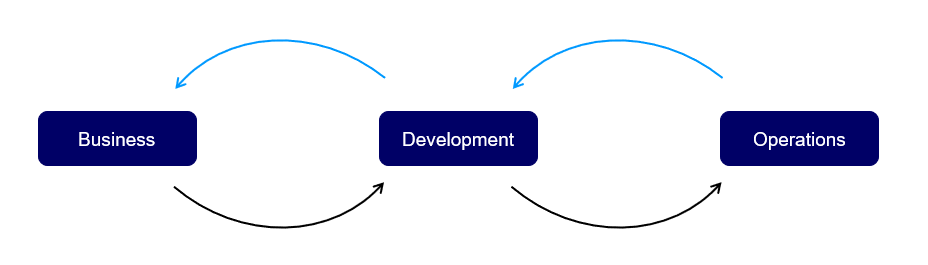
\includegraphics[scale=0.6]{Bilder/Second Way.png}
    \caption{Der zweite Weg: Feedback-Schleifen verstärken \cite{kim_three_2012}}
\end{figure}

Während sich der erste Weg technische und der zweite Weg organisatorische Aspekte beinhaltet, zielt der dritte Weg auf die Etablierung kultureller Änderungen ab um Innovationen weiter voranzutreiben. 

Dieser beschreibt die Schaffung einer Kultur die einen dynamischen Ansatz zum kontniuierlichen Experimentieren und firmenweites Lernen ermöglicht. 

\begin{figure}[h]
    \centering
    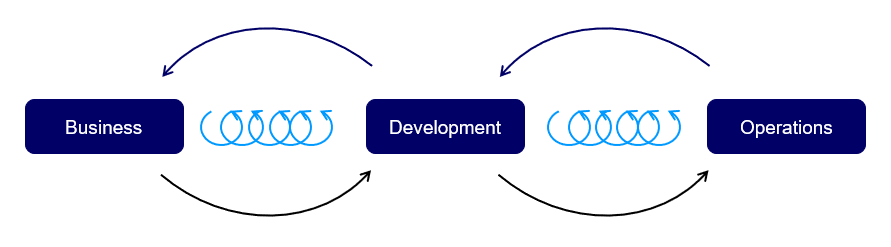
\includegraphics[scale=0.6]{Bilder/Third Way.png}
    \caption{Der dritte Weg: Kultur des kontniuierlichen Experimentierens und Lernens \cite{kim_three_2012}}
\end{figure}

Mittels dieses Ansatzes kann tiefer in die Materie und damit Risiken eingegangen werden, um schwierige oder versteckte Probleme identifizieren zu können. 

Infolgedessen sollen Fehler nicht nur aktiv beseitigt, sondern proaktiv danach gesucht und verbessert werden. \cite[S. 255]{tiemeyer_handbuch_2021}

Für eine erfolgreiche Durchführung des dritten Weges, sollte die etablierte Kultur auf Vertrauen beruhen. 

Je höher der Grad des Vertrauens jedes Mitarbeiters, desto wahrscheinlicher und schneller ist die Weitergabe von gewonnenen Erkenntnissen. \cite[S. 357]{kim_phoenix_2014}

Gemäß der DevOps-Kultur entfällt insbesondere die Bewertung von entdeckten Fehlern, sondern die Möglichkeit von diesen zu lernen und sich zu verbessern, rückt in den Vordergrund. 

Dieser Ansatz steigert die Motivitation jedes Mitgliedes eines DevOps-Teams und fördert das Experimentieren und daraus ableitende Eingehen eines Risikos, wodurch ein globales Lernen ermöglicht wird. 

Zu den Ergebnissen des Dritten Weges gehören die Einplanung von Zeit für die Verbesserung der täglichen Abläufe, die Schaffung von Routinen, die das Team für das Eingehen von Risiken honorieren und die Einbeziehung von Fehlern in das System, um die Belastbarkeit zu erhöhen.


%Durch die Interaktion der beiden Bereiche Development und Operations gehen auch organisatorische Änderungen mit einher, damit eine umfassende DevOps-Kultur geschaffen werden kann. In diesem Abschnitt wird insbesondere auf die Ziele dieser Kultur eingegangen, damit die Zusammenarbeit zwischen den beiden Bereichen gelingt. In diesem Rahmen wird unter anderem auf die wesentlichen Aspekte/Werte wie Kontniuierliches Lernen, Experimentieren, Ingenieurskultur, Kultur der Effektivität, Produktdenken oder die Übernahme von Verantwortung eingegangen. Auch wird der Vergleich und die Nachteile des traditionellen Silodenkens aufgegriffen. 